\documentclass{article}

\usepackage{authblk}
\title{Supplementary Methods, Tables, and Figures}
 \author[1]{Wancen Mu}
 \author[2]{Eric Davis}
 \author[5]{Stuart Lee}
 \author[6]{Mikhail Dozmorov}
 \author[2,3]{Douglas H. Phanstiel}
 \author[1,4]{Michael I. Love \thanks{michaelisaiahlove@gmail.com}}
 \affil[1]{Department of Biostatistics, }
 \affil[2]{Curriculum in Bioinformatics and Computational Biology, }
 \affil[3]{Thurston Arthritis Research Center, Department of Cell Biology \& Physiology, Lineberger Comprehensive Cancer Center, Curriculum in Genetics \& Molecular Biology, and}
 \affil[4]{Department of Genetics, University of North Carolina-Chapel Hill, NC 27599}
 \affil[5]{Genentech, South San Francisco, CA, USA}
 \affil[6]{Department of Biostatistics, Department of Pathology, Virginia Commonwealth University, Richmond, VA 23298, USA}

\date{\today}
\usepackage{graphicx}
\usepackage{graphics}
\usepackage{amsmath}
\usepackage{threeparttable}
\usepackage[top=1in,left=1in,right=1in,bottom=1in]{geometry}
\usepackage[usenames,dvipsnames,svgnames,table]{xcolor}
\usepackage{xspace}
% \usepackage{hyperref}
\usepackage[colorlinks=true,linkcolor=black,citecolor=blue,urlcolor=blue,]{hyperref}
\usepackage{natbib}
\usepackage{xcite}

% cross-ref with main paper
\usepackage{xr}
\makeatletter
\newcommand*{\addFileDependency}[1]{% argument=file name and extension
  \typeout{(#1)}
  \@addtofilelist{#1}
  \IfFileExists{#1}{}{\typeout{No file #1.}}
}
\makeatother
\newcommand*{\myexternaldocument}[1]{%
    \externaldocument{#1}%
    \addFileDependency{#1.tex}%
    \addFileDependency{#1.aux}%
}
\myexternaldocument{plain}


\usepackage[ruled,vlined,linesnumbered,noresetcount]{algorithm2e}
\newcommand\mycommfont[1]{\footnotesize\ttfamily\textcolor{blue}{#1}}
\SetCommentSty{mycommfont}
\usepackage{float}
\usepackage[section]{placeins}
\usepackage[capitalise,noabbrev]{cleveref}
\usepackage{stfloats}
\usepackage{bm}
\usepackage{booktabs}
\usepackage{diagbox} % for diag line in table
\usepackage{hyperref}
\usepackage{geometry}
\usepackage{bm}
\usepackage{amsfonts,amssymb} %font
\usepackage{amsthm}
\usepackage{booktabs}
\usepackage{subfigure}
\geometry{a4paper,scale=0.8}
\renewcommand{\thefigure}{S\arabic{figure}}
\renewcommand{\thetable}{S\arabic{table}}
\renewcommand{\thesubfigure}{\Alph{subfigure}}

\usepackage[utf8x]{inputenc} % deal with "-" not usually set up by the [utf8] option

\newcommand{\code}[1]{\texttt{#1}}
\newcommand{\bootranges}{\emph{bootRanges}\xspace}
\newcommand{\nullranges}{\emph{nullRanges}\xspace}
\newcommand{\granges}{\texttt{GRanges}\xspace}
\newcommand{\plyranges}{\emph{plyranges}\xspace}
\newcommand{\mike}[1]{\textcolor{red}{[Mike: #1]}}
\newcommand{\wancen}[1]{\textcolor{purple}{[wancen: #1]}}


\usepackage{listings}
\lstset{numbers=left, %设置行号位置
        numberstyle=\tiny, %设置行号大小
        keywordstyle=\color{blue}, %设置关键字颜色
        commentstyle=\color[cmyk]{1,0,1,0}, %设置注释颜色
        frame=single, %设置边框格式
        escapeinside=``, %逃逸字符(1左面的键),用于显示中文
        %breaklines, %自动折行
        extendedchars=false, %解决代码跨页时,章节标题,页眉等汉字不显示的问题
        xleftmargin=1em,xrightmargin=1em, aboveskip=1em, %设置边距
        tabsize=4, %设置tab空格数
        showspaces=false %不显示空格
       }
\usepackage{xcolor}

% \geometry{a4paper,left=2cm,right=2cm,top=1cm,bottom=1cm}

\begin{document}

\maketitle

\section{Supplementary Methods}\label{sec:suppmethods}

\subsection{Comparison to previous methods}
In order to generate background feature sets for null hypothesis
testing of association analysis, there are two general categories of methods.  
One method for generating background genomic features sets is to sample from a larger experimental pool or database, like 
LOLA \citep{sheffield2016lola} using Fisher's exact test, and Poly-Enrich \citep{lee2020poly} using likelihood ratio test based on negative binomial likelihood. 
Another method is to permute or shuffle the genomic ranges, giving
random start sites to existing features, possibly considering an
exclusion list of regions where features should not be
located. Examples of this type of method include 
bedtools \citep{quinlan2010bedtools}, ChIP-Enrich
\citep{welch2014chip}, or
GenometriCorr \citep{GenometriCorrfavorov2012}.
GAT additionally allows controlling for GC content \citep{GAT_2013},
and regioneR also implement a circular randomization to preserve
inter-feature distance \citep{gel2016regioner}.
Our methods are similar to the second type, in that we redistribute
features along the genome, but we preserve inter-feature distances, as
in regioneR, but using a block resampling scheme, as in GSC
\citep{bickel2010subsampling}.

\subsection{Segmentation formulation}
In the following we define variables for genome segmentation and use the notation as defined by \citep{bickel2010subsampling}.
From Ensembl annotation databases, we can obtain the position of all
genes, so that we can compute
gene density as the count of genes per million basepairs. Suppose original sequences are $\{X_1,...,X_n\}$
and we assume there exist integers
$\bm{\tau}=\bm{\tau^{(n)}}=(\tau_0,...,\tau_U)$, where $0=\tau_0 <
\tau_1 < ... <\tau_U = n$, such that the collections of variables,
${\bm{X}_{\tau_i},...,\bm{X}_{\tau_{i+1}}}$, are separately stationary
for each $i=0,...,U-1$. Here stationary means more homogeneous in their feature density.
We let $n_i=\tau_i-\tau_{i-1}$ be the length
of the \textit{i}th region. Hence, we introduce the
mapping $$\pi:\{1,...,n\}\rightarrow\{(i,j):1\leq i \leq U,1\leq j
\leq n_i\},$$ which relates the original sequence $\{X_1,...,X_n\}$ to
the segmentation sequence $\{X_{ij}:1\leq i \leq U,1\leq j \leq n_i\}$.

We considered various genome segmentation procedures or annotations in the paper, e.g. Circular Binary Search (CBS) \citep{cbs}, HMM \citep{rcpphmm}, and published segmentations(Roadmap). CBS and HMM are implemented as a built-in function in \nullranges as follows. We tile the genome based on segmentation length ($L_s$, e.g. on the order of ${\sim}1$ Mb) first and derive the gene density within each tile genome. CBS will recursively splits chromosomes into either two or three subsegments of estimated equal gene density and then use kmeans to cluster the subsegments. While HMM will model the gene density by a multinomial distribution given the number of hidden states and use Viterbi algorithm for hidden state decoding. Roadmap segmentations derived by ChromHMM \citep{ernst2012chromhmm} were downloaded from \url{https://egg2.wustl.edu/roadmap/web_portal/}. ChromHMM is based on a multivariate Hidden Markov Model that explicitly models the presence or absence of each chromatin mark. It generated segmentation including 15 small states and we summeraized them into 3 big categories: low density("E9","E13","E14","E15"), middle density("E10","E11","E12"), high density("E1-E8"). 8,797 ranges left after merging states and mean width was around 0.33Mb. 

\subsection{Shuffling}\label{sec:shuffle}
Genome shuffling was performed by random sample SNPs in acceptance region on Genome with probability proportional to SNPs count on each chromosome. The acceptance region excluded all ENCODE excludable regions plus telomere,centromere from UCSC and rCGH derived from \code{excluderanges} for hg38 \citep{excluderanges}.


\subsection{Assessment of \bootranges}
Suppose we are interested in region overlap between one feature $\bm{x}$, denoted by $T_1, ..., T_\alpha$ with lengths $\tau_1,..., \tau_\alpha$, and the feature $\bm{y}$, denoted by $Q_1, ..., Q_\beta$ with lengths $\rho_1, ..., \rho_\beta$, then the region overlap is defined as $s_{obs} \equiv  \frac{1}{\alpha}\sum_{t=1}^\alpha V_t$ where $V_t=1-\prod_{k\in (T_t+\theta)}(1-J_k)$ and $J_k=1$ if position $k$ belongs to feature $\bm{y}$ and 0 otherwise. $\theta$ is the shift among feature $\bm{x}$ and $\bm{y'}$, such as 1kb when linking promoters to gene. After we do the block bootstrap according to the segmentation region, we generate $R$ new sets of null features $\bm{y'}$ and $R\times \frac{n}{L_b}$ blocks. Therefore, we can do both genome-wise or block-wise analysis based on the question being addressed. Either using $s_{1}, s_{2}, ..., s_{R}$ to derive empirical \textit{p}-value $=  \frac{1}{R} \sum_{r=1}^R \mathbb{I}_{\{s_r > s_\text{obs}\}}$ or $s_{1}, s_{2}, ..., s_{R\times \frac{n}{L_b}}$ to derive empirical \textit{p}-value $=  \frac{1}{R\times \frac{n}{L_b}} \sum_{r=1}^{R\times \frac{n}{L_b}} \mathbb{I}_{\{s_r > s_{obs}\}}$. Additionally, we could used the $z$ score to measure the distance between the observed statistics and the bootstrap statistics distribution in terms of standard deviations. Specifically, the z score in \cref{fig:result} is calculated by $$z = \frac{s_\text{obs} - \widehat{s}}{ \text{sd}_R(\widehat{s})},$$ where $\widehat{s} = \frac{\sum_{r=1}^R \widehat{s_r}}{R}$ is the sample mean of the $R$ replications and $\text{sd}_R(\widehat{s}) = \sqrt{\frac{\sum_{r=1}^R [\widehat{s_r}-\widehat{s}]^2}{R-1}}$.
Note that, if block-wise analysis is preferred, the SD of bootstrap distribution should be scaled by $\sqrt{L_b}$.




% $$P_{H_0}[R_n\geq r_{n}]\approx 0.05$$

\subsection{Swaping algorithm}\label{sec:algorithm}


% \begin{algorithm}
% \SetNoFillComment
% \caption{Block bootstrap GRanges across chromosome} \label{alg:supp_unseg}
%   \KwData{Feature GRanges, Block length($L_b$), bootstrap times(R), type('permute' or 'bootstrap')}
% \KwResult{Bootstrapped distribution of test statistics}
% \While{r \leq R}{
% \textbf{rearranges block:} Generate consecutive tiling blocks with width = $L_b$ \tcp*[l]{where 'bait' blocks will be moved} \\
% \uIf{permutation}{
% \textbf{random block:} Sample blocks without replacement from \textbf{rearranged block} \\
% }\ElseIf{bootstrap}{ 
%          $n_b = \sum_{j=1}^{24} ceiling(L_{c} / L_b)$\\
%          \textbf{random block:} Generate $n_b$ blocks with replacement and probability weights proportional to $L_c$ \tcp*[l]{these blocks are the 'bait' for capturing features in $\bm{y}$}\\}
% Find overlap of random blocks and feature $\bm{y}$ \tcp*[l]{use the bait to sample features in $\bm{y}$}\\
% Swap the ranges in those bait blocks given the shift between random block and rearranged block} \\
% Bind bootranges object which has $r$ and $L_b$ as metadata columns $\gets$ plyranges.
% \end{algorithm}


\begin{algorithm}[H]
  \SetAlgoLined
  \KwData{Feature GRanges ($\bm{y}$), Block length ($L_b$), Length of chromosome $c$ ($L_c$), Total number of choromosome ($C$), Bootstrap times ($R$), Type(`permute' or `bootstrap')}
  \KwResult{$\bm{bootRanges}$ object, a GRanges object with all the ranges concatenated, and iteration and block length indicated by metadata columns}
  \While{$r \leq R$}{
    \textbf{rearranged blocks:} Generate consecutive tiling blocks with width = $L_b$\\% \tcp*[l]
    \uIf{permutation}{
\textbf{random blocks:} Sample blocks without replacement from rearranged blocks
}\ElseIf{bootstrap}{ 
         $n_b = \sum_{c=1}^{C} \text{ceiling}(L_c / L_b)$\\
         \textbf{random blocks:} Generate $n_b$ blocks with replacement and number of blocks per chromosome is proportional to $L_c$\\ %\tcp*[l]
      }
%Find overlap of random blocks and feature $\bm{y}$\\% \tcp*[l]
Move featues in $\bm{y}$ that fall into random blocks to rearranges blocks given the shift as difference between random blocks and rearranged blocks start sites
}
\caption{Block bootstrap GRanges across chromosome} \label{alg:supp_unseg}
\end{algorithm}



\begin{algorithm}
\SetNoFillComment
\caption{Segmented block bootstrap with proportional block length}\label{alg:framework}
  \KwData{Feature GRanges($\bm{y}$), Block length ($L_b$), Length of total genome ($L_C$), Bootstrap times ($R$), Segmentation GRanges with $L_j$ represents each ranges width and $\alpha_i$ represents ranges belong to state $i$}
  \KwResult{$\bm{bootRanges}$ object, a GRanges object with all the ranges concatenated, and iteration and block length indicated by metadata columns}
\While{$r \leq R$}{
\For{each segmentation state $i$}{
        $L_s^i = \sum_{j\in \alpha_i} L_j$ \\
         $L_b^i = L_b * L_s^i / L_C$ \\
         $n_b^i = \sum_{j\in \alpha_i} \text{ceiling}(L_{j} / L_b^i)$ \\
	\textbf{rearranged blocks:} Generate $n_b^i$ tiling blocks start site \\
         \textbf{random blocks:} Generate $n_b^i$ blocks start site with replacement and and number of blocks per ranges is proportional to $L_j$ \\
         \textbf{Return:} rearranged and random  block start and chromosome names
    }
Construct random blocks Granges\\
Move featues in $\bm{y}$ that fall into random blocks to rearranged blocks given the shift as difference between random blocks and rearranged blocks start sites
}
\end{algorithm}

\begin{algorithm}
\SetNoFillComment
\caption{Segmented block bootstrap with fixed block length across chromosome}\label{alg:supp_fixedlb}
  \KwData{Feature GRanges($\bm{y}$), Block length ($L_b$), Length of total genome ($L_C$), Bootstrap times ($R$), Segmentation GRanges with $L_j$ represents each ranges width and $\beta$ represents total number of ranges}
  \KwResult{$\bm{bootRanges}$ object, a GRanges object with all the ranges concatenated, and iteration and block length indicated by metadata columns}
\While{$r \leq R$}{
         $n_{j} = \text{ceiling}(L_{j} / L_b)$ \\
         $n_b = \sum_{j=1}^{\beta} n_j$ \\
         \textbf{rearranges blocks:} Generate $n_b$ tiling blocks start site by order with width = $L_b$  \\
 	\textbf{random blocks:} Generate $n_b$ blocks start site with replacement and number of blocks per ranges is proportional to $L_j$ \\
\For{each segmentation state $i$}{
         Identify rearranged blocks that are in state $i$  \\
	Identify random blocks that are in state $i$ \\
         \textbf{Return:} random block start sites and chromosome names, rearranged block start sites and chromosome names
    }
Construct random blocks Granges \\
Move featues in $\bm{y}$ that fall into random blocks to rearranged blocks given the shift as difference between random blocks and rearranged blocks start sites
}
\end{algorithm}



% \input{dataprocess}\label{section:preprocessing}

\section{Supplementary Results} \label{sec:results}
\subsection{Liver caQTL-GWAS colocalizations}
1872 SNPs data were download from the NHGRI-EBI GWAS catalog \citep{gwascatalog} on September 22, 2021. We only extracted single variant  associated with total cholesterol. Liver ATAC-seq
\citep{CURRIN20211169} information of 20 samples were downloaded from GSE164870.
Then genomic coordinates of consensus peaks were converted from hg19 to hg38 using \code{liftOver} to construct 221,606 peaks GRanges.

\subsubsection{$L_b$ selection}\label{sec:length}
On the issue of 
block length selection, we considered it in two ways. One is trying to find $L_b$ that has the minimum value of a pseudometric $d^*(v)=|\sqrt{\frac{L_{v-1}}{L_v}}\text{IQR}(\mathcal{L}_{L_v})-\text{IQR}(\mathcal{L}_{L_{v-1}})|$ where $\mathcal{L}_{L_v}$ is the statistic distribution at length $L_v$, $v=1,2,\cdots,V$, and $V$ is the number of candidate block lengths and $\text{IQR}(\mathcal{L})$ is the interquartile range of statistics distribution following \citet{bickel2010subsampling}. \cref{fig:suppfig0}A showed $d^*$ were in common had smaller values when $L_b\in[300000,800000]$. The second way is evaluating conserved spatial pattern that generated null sets have similar properties with original sets, eg. inter-feature distance. We used the Earth's Mover distance (EMD) to quantify the similarity between the distributions of an inter-feature distance in the original  and  null  dataset,  resulting  in  values  between  zero  (identical  distributions)  to  one  (totally  disjoint  distributions). The EMD between two distributions is proportional to the minimum amount of work required to change one distribution($y$) into the other($y'$). Here $y$ and $y'$ is the histogram of original and null inter-feature distance with bin size = 0.3. Since the EMD always decreased as $L_b$ increased because more neighbouring features reserved, the right $L_b$ should be chosen so that longer length doesn’t improve much as well as it is much smaller than the $L_s$. So,[200000,600000] was shown to be  a good range by visualization and according to the Elbow Method of EMD (\cref{fig:suppfig0}B-C). 


\subsection{Macrophage cell lines}\label{sec:splines}
Processed 24 macrophage samples' RNA-seq  and 145 samples' ATAC-seq were loaded from \code{fluentGenomics}\citep{lee2020fluent}. They were measured after interferon gamma(IFNg) stimulation. Since the transcriptomic response to IFNg stimulation may be mediated through an increasing transcription factors bindings on nearby regions and ATAC-seq can captioned those regions' accessibility, we expect there would have an enrichment of differentially accessible (DA) ATAC-seq peaks in the vicinity of differentially expressed (DE) genes. 

When performing block bootstrap with 500kb block length on 100 times, we got $z_{99}=-108.1$ and $\textit{p}$-value $<.05$. We rejected the null hypothesis and concluded that there was significant enrichment of DA peaks near DE genes by finding overlaps.

For fitting the generalized penalized splines, \code{gam} function in the \code{mgcv} package was used to fit the model, which was based on a penalized likelihood maximization, and generalized cross-validation was utilized to choose the optimal value for the smoothing parameter, $\lambda$. Then, \code{tidymv} package was implemented to predict and extract the fitted value. 

\begin{lstlisting}[language=R]
boot_stats <- x %>% plyranges::join_overlap_inner(bootRanges) %>%
  plyranges::group_by(id.x,iter) %>%
  plyranges::summarize(count = plyranges::n(), logFC = max(logFC)) %>%
  as.data.frame() %>%
  tidyr::complete(`id.x`, iter, fill=list(count = 0)) %>%
  dplyr::select(iter, count, logFC) %>%
  tidyr::nest(-iter) %>%
  dplyr::mutate(
	 fit= map(data, ~gam(count ~ s(logFC), data = ., family=poisson)),
         pred  = map(fit, ~predict_gam(model = ., length_out = 2000)),
         fitted = map(pred,~find_fit(data=., logFC = seq(-8,10,1))))

\end{lstlisting} 

\subsection{Chromium Single Cell Multiome ATAC + Gene Expression assay}
Data were downloaded according to \citet{Vignette} which includes genes and peaks in 10,032 cells. Cell type annotations have been done as a priori by the 10x Genomics R\&D team. Then information on chromosome 1 to 22 were selected to construct gene and peak GRanges. Since the main goal is not to accurately find gene-promoter pairs but the realization, the following preprocess may not be the most suitable way. First, we aggregated cells within same cell types, to form ‘pseudobulks’ with 14 samples according to the metadata because psuedobulking provided smoother correlation statistics without loss of the information of interest. Next, we removed all the features with 0 standard deviation. Then, log counts per million (CPM) were computed from \code{edgeR} for accounting for different library size.

Since genes' expression is most \textit{cis}-regulated by chromatin accessibility, there is a belief that two modalities would have significant high correlation. And extremely high expressed or low expressed genes would also have high or low accessibility in corresponding cell types. For the whole gene set, the mean correlation of genes and ATAC-seq read counts was 0.33, while the subsampling correlation distribution in \cref{fig:suppfig3} A had mean 0.007 across 1000 times block bootstraps. Additionally, the average gene-peaks correlation per gene can be
computed and compared to a bootstrap distribution to
identify 5644 gene-promoter pairs that were significantly correlated across cell types, among which 5591 genes had only
one pair, 25 genes had 2 pairs. 
% The most negative correlation gene TET3 has $\rho = -0.963$\cref{fig:suppfig}G outside the subsampling confidence interval [-0.85,0.78] and previous studies have assessed down-regulation TET3 are essential for B-cell development and tumorigenesis\citep{lio2019dysregulation}. Similarly, CD83\cref{fig:suppfig}H with $\rho = 0.992$ outside [-0.80, 0.68] was a well known myeloid markers\citep{li2019cd83}. 
Those significant pairs could provide important insights into perturbation experiments for validation. Two examples were shown in \cref{fig:suppfig3}B-C. The block below shows example code for running analysis.
\begin{lstlisting}[language=R]
# split sparse count matrix into NumericList
x <- x_Granges %>%
  mutate(counts_X = NumericList(asplit(x.cpm, 1)))%>% sort()
y <- y_Granges %>%
  mutate(counts_y = NumericList(asplit(y.cpm, 1))) %>% sort()
# First standardize read counts for fast correlation computation
x$counts1 <- NumericList(lapply(x$counts_X,function(z)(z-mean(z))/sd(z)))
y$counts2 <- NumericList(lapply(y$counts_y,function(z)(z-mean(z))/sd(z)))

bootranges <- bootRanges(y,blockLength = 5e5, R=100)
  
# for standardized x and y:
correlation = function(x,y) 1/(length(x)-1) * sum(x*y)
## extract bootstrap summary statistics
boot_stats<-x %>% plyranges::join_overlap_inner(boots, maxgap=1000) %>%
  plyranges::mutate(rho = correlation(counts_x, counts_y)) %>%
  plyranges::group_by(iter) %>%
  plyranges::summarise(meanCor = mean(rho)) 
\end{lstlisting} 
 
\newpage
\section{Supplementary Figures}
\begin{figure*}[htbp]
\centering
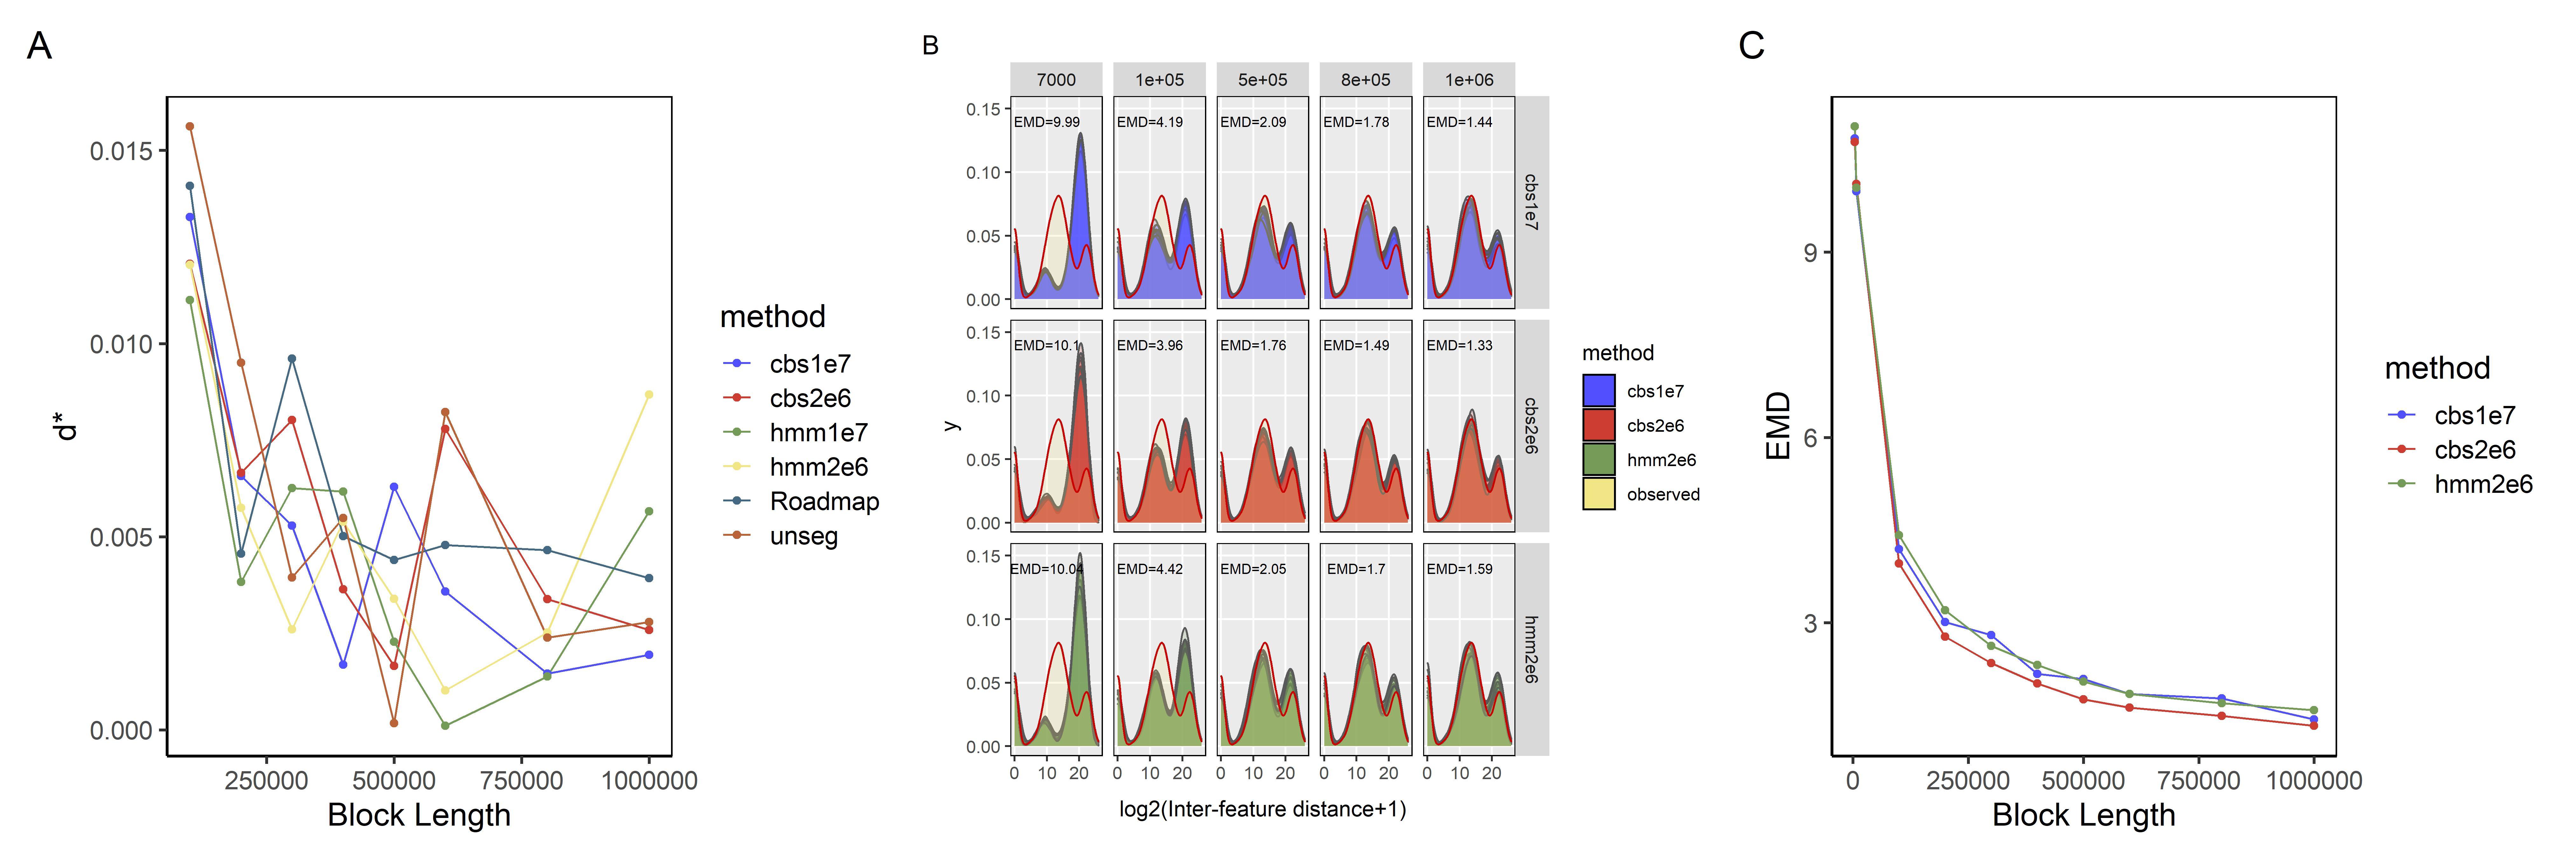
\includegraphics[scale=0.35]{Figures/sfig1.jpeg}
\caption{$L_b$ selection assesment. A) A pseudometric $d^*$ over $L_b$, B) The null sets' log2(inter-feature distance+1) density plots generated by various block bootstrapped settings over observed feature set's log2(inter-feature distance+1) distance. The more null sets' density plots overlapped with observsed features, the better conversing spatial distribution of original set captured by block bootstrapped. Median EMD were shown as text in each panel. C) Median EMD over $L_b$ where EMD quantified similarity between two distributions. } 
\label{fig:suppfig0}
\end{figure*}

\begin{figure*}[htbp]
\centering
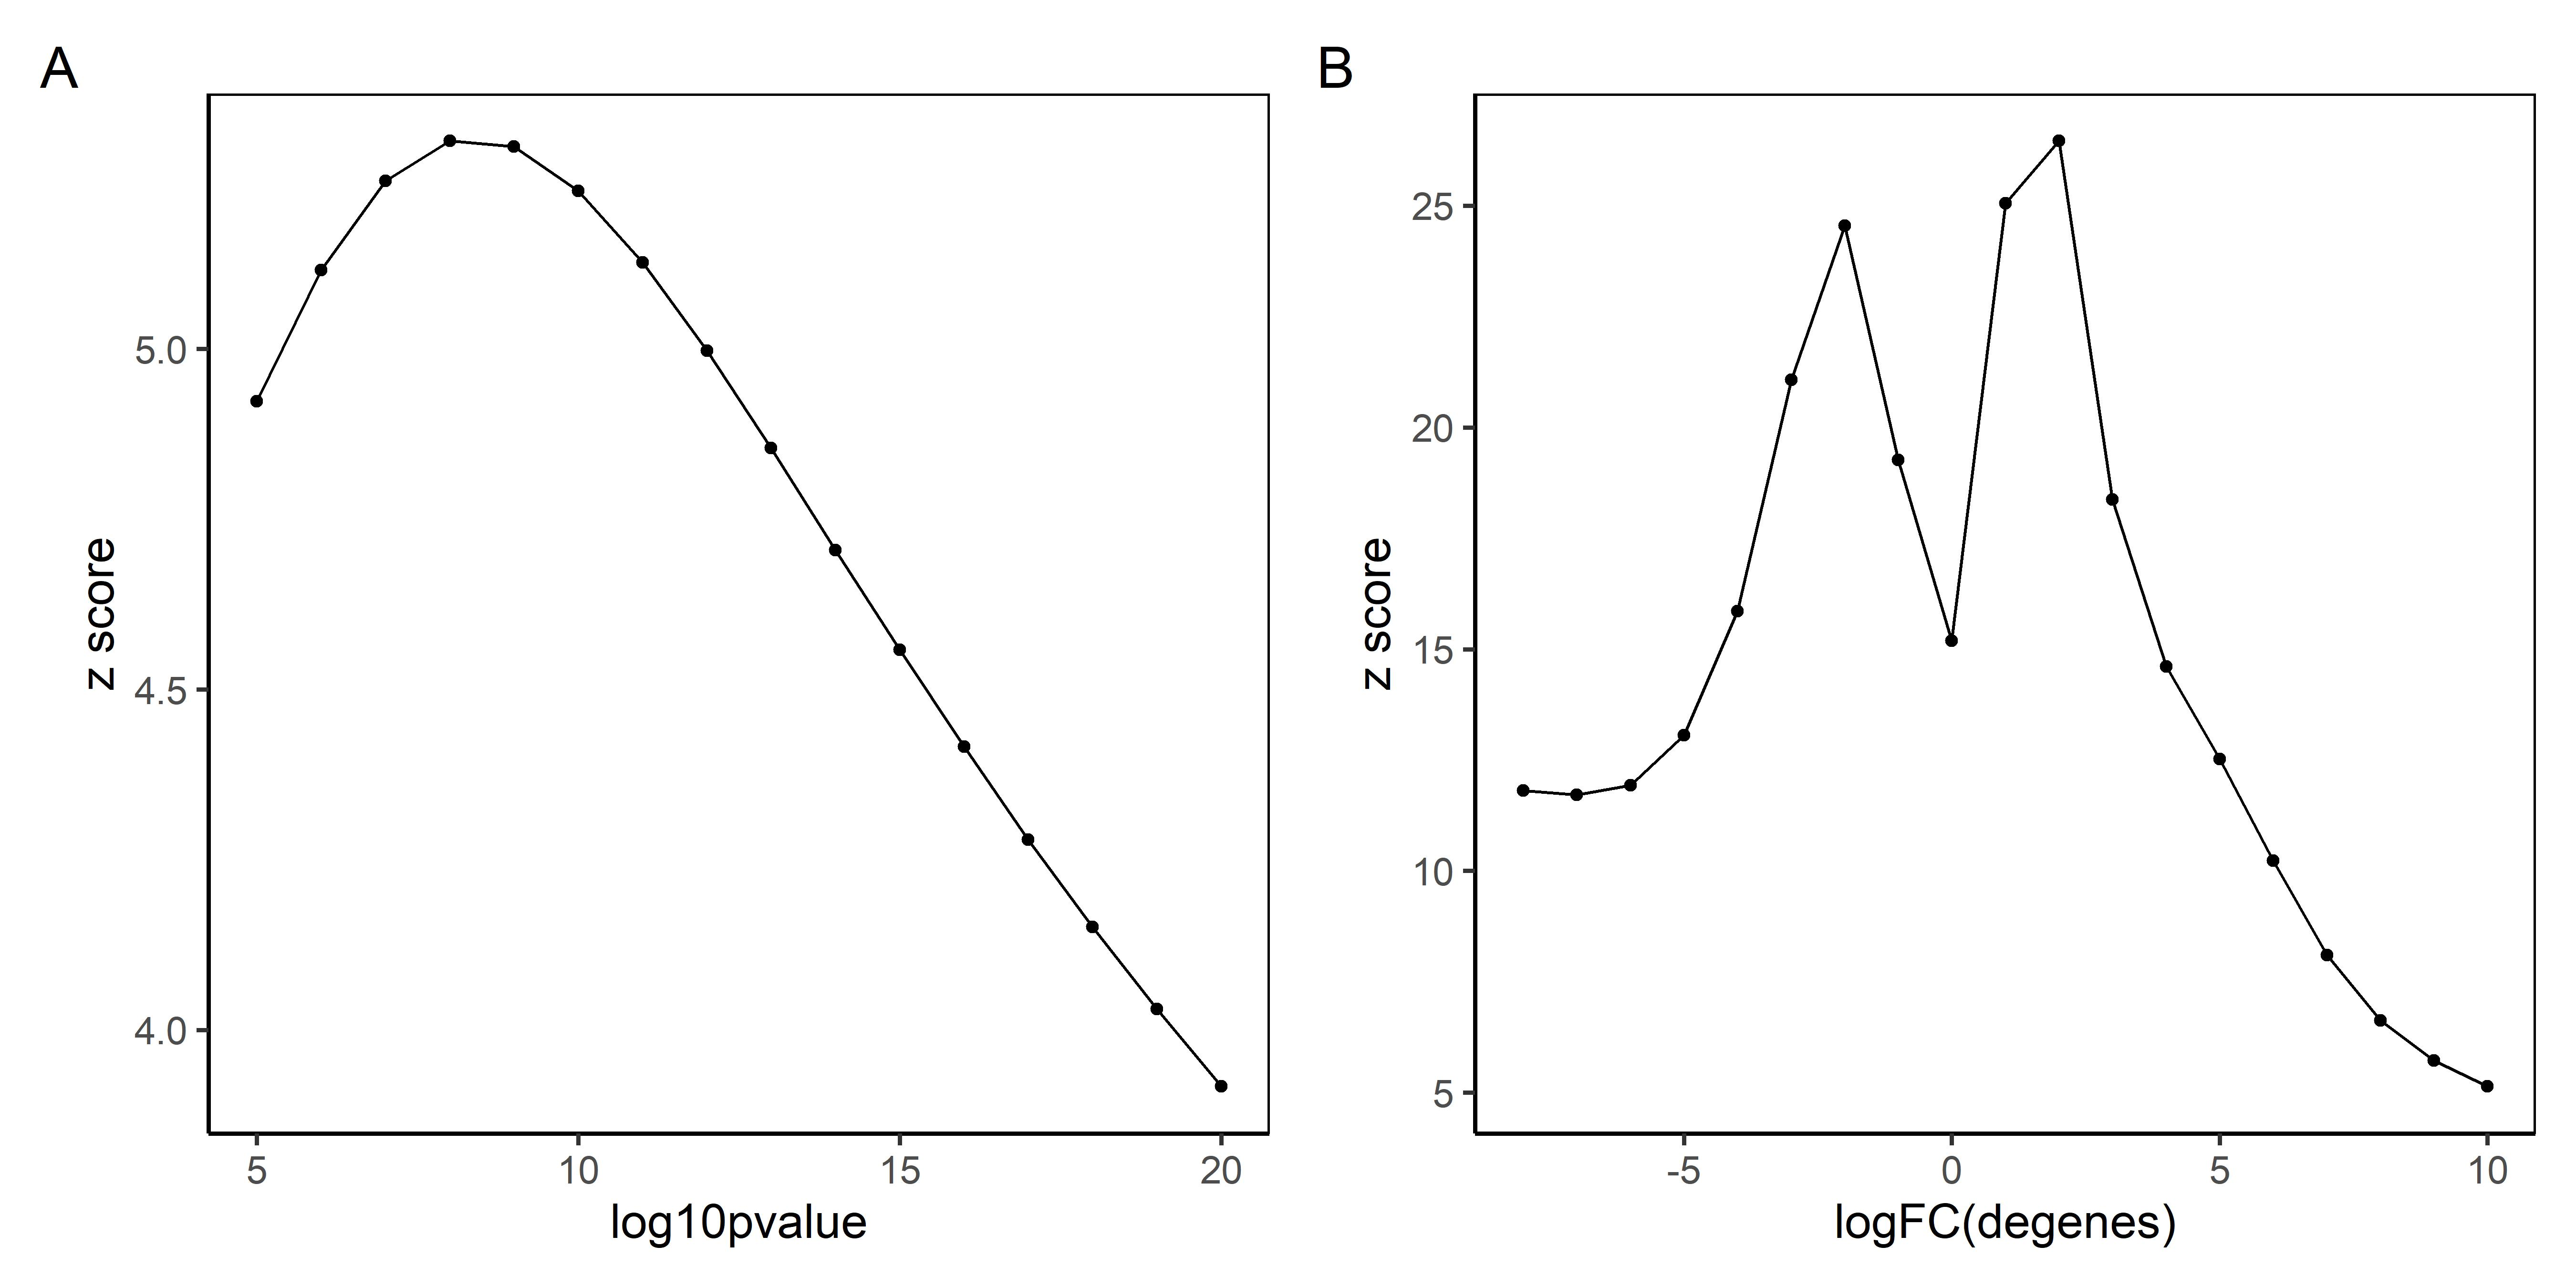
\includegraphics[scale=0.3]{Figures/zscore.jpeg}
\caption{ A)\textit{z} score over -log10(pvalue) on the liver dataset. B) \textit{z} score over DE genes' logFC on the macrophage dataset. \textit{z} score indicated the amount of standard deviations that observed fitted overlap count away from 1000 times block bootstrap's fitted overlap count.} 
\label{fig:suppfig2}
\end{figure*}

\begin{figure*}[htbp]
\centering
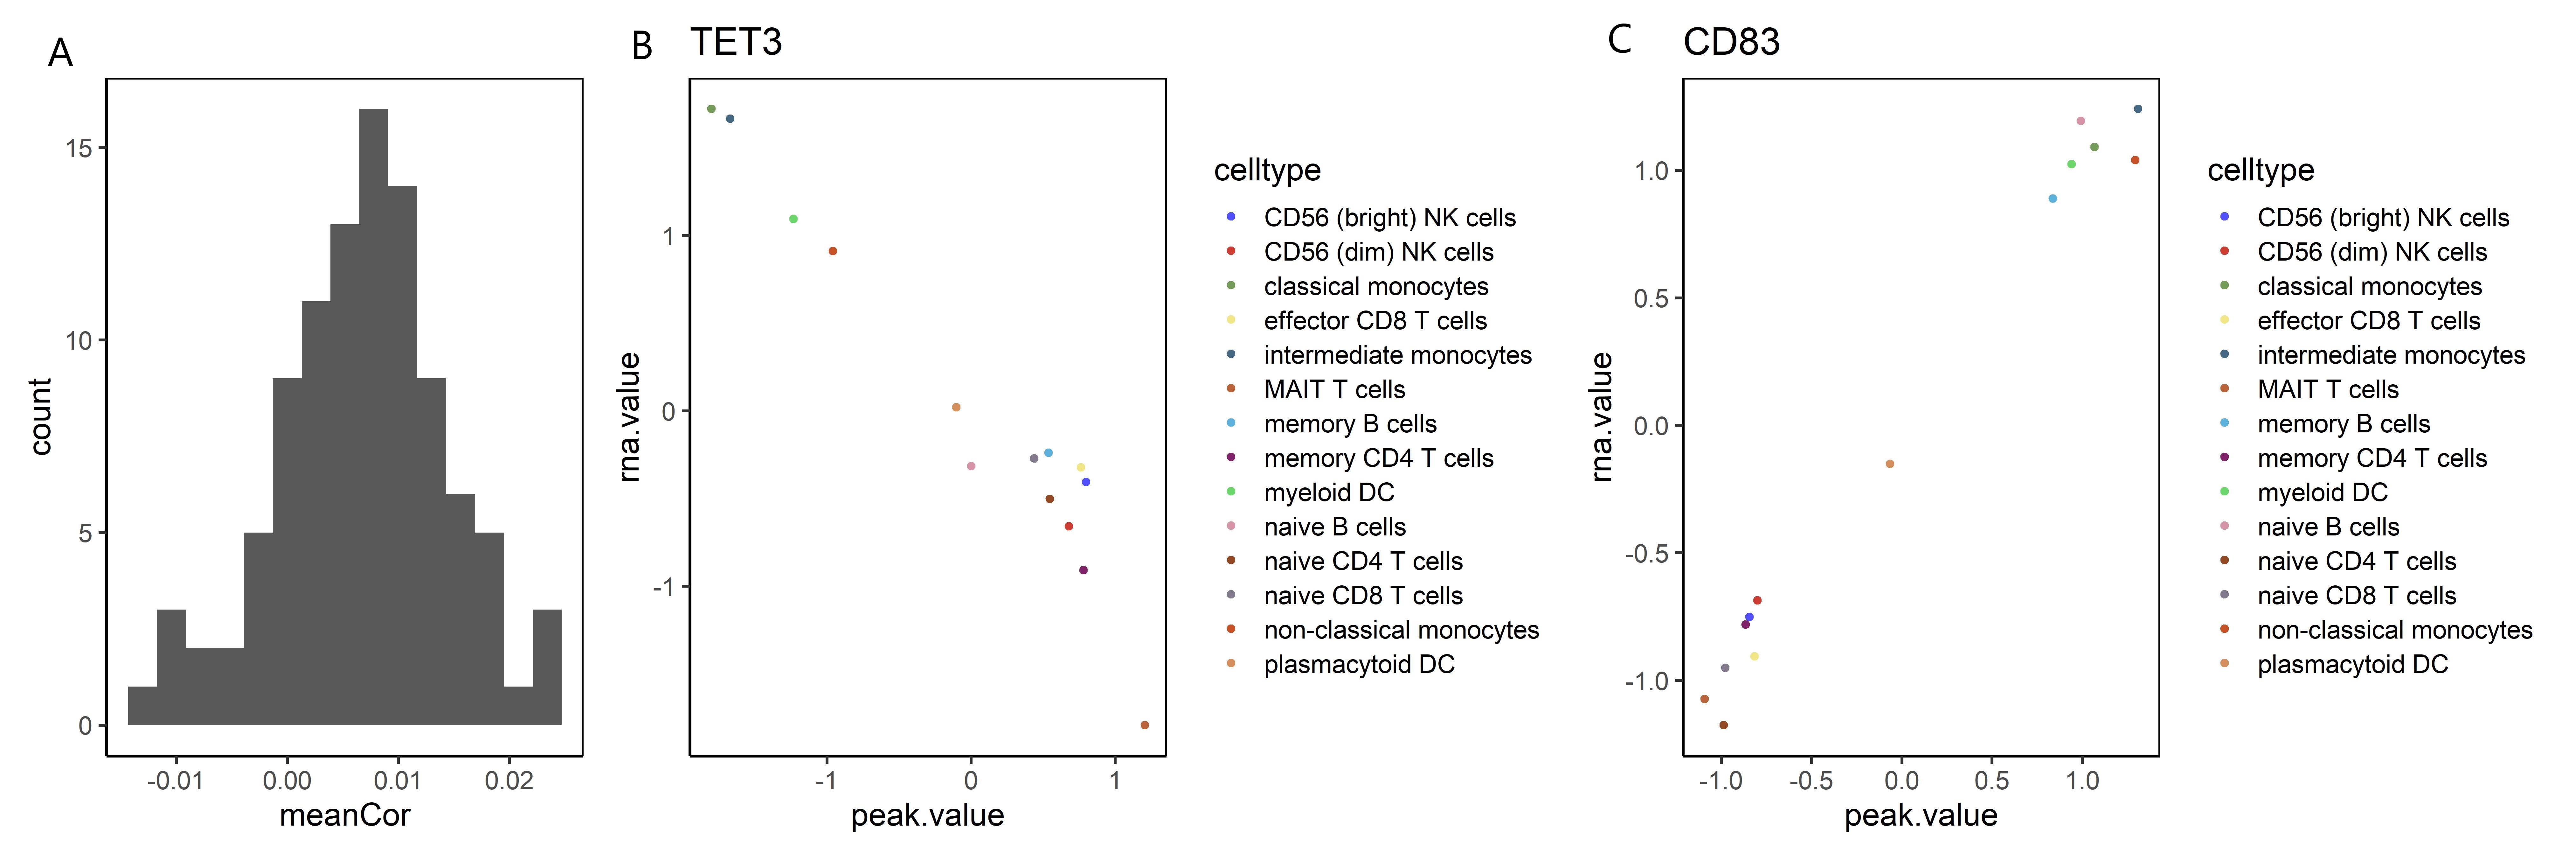
\includegraphics[scale=0.08]{Figures/sfig2.jpeg}
\caption{Results of Chromium Single Cell Multiome ATAC + Gene Expression assay. A)The mean correlation distribution of genes expression with 1000 times block bootstrapped ATAC's read counts. B) Gene TET3 read counts over peak chr2:74000098-74003475 read counts, colored by cell types. TET3 has the most negative correlation $\rho = −0.963$. C) Gene CD83 read counts over peak chr6:14116971-14139988 read counts, colored by cell types. The correlation of this gene-promoter pair is 0.992.} 
\label{fig:suppfig3}
\end{figure*}

\bibliographystyle{natbib}
%\bibliographystyle{achemnat}
%\bibliographystyle{plainnat}
%\bibliographystyle{abbrv}
%\bibliographystyle{bioinformatics}
%
%\bibliographystyle{plain}
%
\bibliography{document}

\end{document}
